 \documentclass[../ewet_cwc_report.tex]{subfiles}

\begin{document}

\section{Electrical Design and Controls}
\subsection{Introduction}

\noindent
In the small-scale turbine design, it is critical to identify
the type of the generator that would be used through the
design process because mechanical designs and modeling are
time consuming and constrained by the academic year's available
man hours. It is important to limit complete change of design
course to one or two instances and even that is only affordable
at the initial stage of the design. The team did not have a
ready generator solution from previous project and had no
practical experience in assessing the scale or the needed
parameters in selecting the generator for such a miniature
design. The only notion that was passed down from previous
team was the understanding of the electrical motor KV rating
and importance of minimizing cogging torque at cut in speed.
Thus, these became the starting point parameters in the
generator selection. The team has encountered several
challenges over the power electronics selection process.
Ideas have been tried and discarded, some because component
selection process was not taking into the account the
component's self-power demand, others because the nature of the
component's operation was not fundamentally understood. In some
instances, where a solution was not found by direct approach,
like in voltage regulation attempts, the team has paused on that
front and shifted attention to better understood sections of the
design, allowing for continuous progress. This approach proved
to be very effective, and more elegant and natural solutions
were found as a result.

\subsection{Generator and Load}

\noindent
Faraday's Law indicates that \emph{``Any change in the magnetic
  environment of a coil of wire will cause a voltage (emf) to be
  induced in the coil''}. Formulation \eqref{eq:emf} demonstrates
the physical relationship described by Faraday using
mathematical interpretation,

\begin{equation}
  \text{emf} = -N \frac{\Delta \phi}{\Delta t}
  \text{\,,}
  \label{eq:emf}
\end{equation}

\noindent
where $N$ represents the number of turns in the coil,
$\Delta\phi$ represents a change in magnetic flux over time,
and $\Delta t$ is the change in time.

Magnetic flux is given by formulation \eqref{eq:flux},
\begin{equation}
  \phi = BA \sin\theta
  \text{\,,}
  \label{eq:flux}
\end{equation}

\noindent
where $B$ representing magnetic field produced by opposing
permanent magnets of the rotors, $A$ represents area of the
coiled wire in the stator and $\theta$ represents the angle
between the coil area plane and the magnetic field and since
the coil area and the magnetic field are orthogonal to each
other in the AFPMG.

Formulation \eqref{eq:flux} can be restated as
\begin{equation}
  \phi = BA
  \text{\,.}
  \label{eq:flux-simple}
\end{equation}

According to Lenz's law, the negative sign of
\eqref{eq:emf} indicates that the current produced by the
change in magnetic flux creates its own magnetic field that
opposes the change in flux that produced it. When applying this
notion to a generator this indicates that current induced in the
generator coils will provide an opposing force to the one that
is responsible for the rotation of the generator shaft. Since
the force is rotational it could be restated in terms of opposing
torque $\tau_G$ and compared against aerodynamic torque
$\tau_W$ extracted from the wind,

\begin{equation}
  \tau_W = \frac{P_W}{\omega_{rotor}}
  = \frac{\rho\pi R^3 C_p\paren{\lambda, \theta} V_W^2}{2\lambda}
  \text{\,,}
  \label{eq:tau-wind}
\end{equation}
where $P_W$, in watts, is the power available in the wind and
is given by \eqref{eq:power-wind}, $\omega_{rotor}$ is the
rotational speed in (\unit{rad\per\s}), $\rho$ is the air
density in (kg / m3), $C_p$ is the power coefficient expressed
as a function of the tip speed ratio and pitch angle and is
given by Eqs. \eqref{eq:tau-r} and \eqref{eq:lambda-i}:

\begin{equation}
  P_w = \frac{\rho\pi R^2 C_p\paren{\lambda, \theta} V_W^2}{2}\
  \text{\,,}
  \label{eq:power-wind}
\end{equation}

\begin{alignat}{3}
  \tau_R & = \frac{P_W \times C_p}{\omega_{rotor}}
  C_p\paren{\lambda, \theta}                               \\
         & = 0.22\paren{\frac{116}{\lambda_i} - 0.040 - 5}
  e^\frac{-12.5}{\lambda_i}
  \text{\,,}
  \label{eq:tau-r}
\end{alignat}

\begin{equation}
  \lambda_i = \paren{\frac{1}{\lambda + 0.8} -
    \frac{0.035}{\theta^3 + 1}}^{-1}
  \text{\,.}
  \label{eq:lambda-i}
\end{equation}

In Equation \eqref{eq:power-wind}, $R$ is the wind turbine
rotor radius in meters, $V_W$ is the wind velocity in
\unit{\meter\per\s}, and $\lambda$ is the tip speed ratio (TSR)
given by Equation \eqref{eq:lambda},

\begin{equation}
  \lambda = \frac{R \omega_{rotor}}{V_W}
  \text{\,.}
  \label{eq:lambda}
\end{equation}

It could be further inferred that wind turbine operation could
be imagined as a system of two opposing torques $\tau_W$ and
$\tau_G$ whenever torques are equal the system is in
equilibrium and is generating constant power. Any time
$\tau_W$ changes in response to change in $V_W$, (for the
experimental environment $\rho$ is assumed constant) there
exists a new equilibrium state of $\tau_W$ and $\tau_G$
torques. Simply put, anytime $V_W$ increases it creates
conditions for a new and greater power equilibrium state, this
means the resistance of the load could be decreased, which will
increase the current flow, and thus more power could be
extracted from the wind.

The KV rating of the generator is responsible for predicting
the magnitude of the generated voltage as a function of the
rotor speed. In the wind turbine controls it is sometimes
important to maintain relatively low rotational speed and at
the same time maintain voltage magnitude that is high enough to
keep the microcontroller active. Equations \eqref{eq:KV} and
\eqref{eq:RPM-KV} show this relationship,

\begin{equation}
  \text{KV}_{rating} = \frac{\text{rotor speed}}{\text{voltage}}
  \text{\,,}
  \label{eq:KV}
\end{equation}

\begin{equation}
  V = \frac{\text{RPM}}{\text{KV}_{rating}}
  \text{\,.}
  \label{eq:RPM-KV}
\end{equation}

Cogging torque is a magnetic interaction between the iron teeth
of the stator and magnets of the rotor in a brushless DC motor
for instance. The team did not know how to assess the magnitude
of such torque and its effect on the cut in speed of the future
turbine so naturally attempts were made to find a motor with
little to no cogging torque. This led to the discovery of the
axial flux permanent magnet motor (AFPMM) which could be used
as a three phase DC generator if coupled with a three-phase
full rectifier circuit.

Figure \ref{img:stator_rotor} shows the single rotor and the
stator of the 12 pole 9 coil AFPMG used in the prototype. A set
of two motors were purchased for initial evaluation of the KV
rating. Using dynamometer, it was experimentally determined
that the KV rating of the single motor was 96. This was very
low comparing to all other available options that also had the
appropriate dimensional scale. Evaluating the mechanical
construction of the motor's design, it was observed that it
appeared to be relatively simple to create a stack of these
motors coupled by a single axle. Once the team recognized the
flexibility in the connection schemes, ability to reduce the
KV rating to 24 by stacking motors on the single axle, and the
virtual absence of cogging torque in this design, two more
motors were immediately ordered.
\begin{figure}[th]
  \centering
  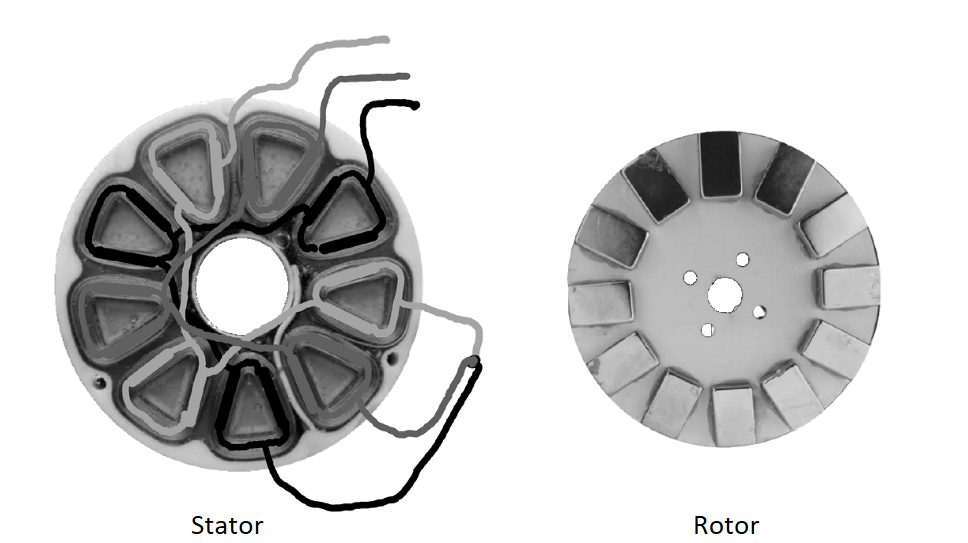
\includegraphics[width=0.4\textwidth]{../_images/stator_rotor.png}
  \caption{Stator and rotor}
  \label{img:stator_rotor}
\end{figure}

Figure \ref{img:housing} demonstrates the midterm version of
the generator design. The housing assembly consists of five
main parts: (b and c) front and back bearing supports,
(d) housing block, (e) stabilizer bar, and (f) yaw pivot
assembly.

\begin{figure}[th]
  \centering
  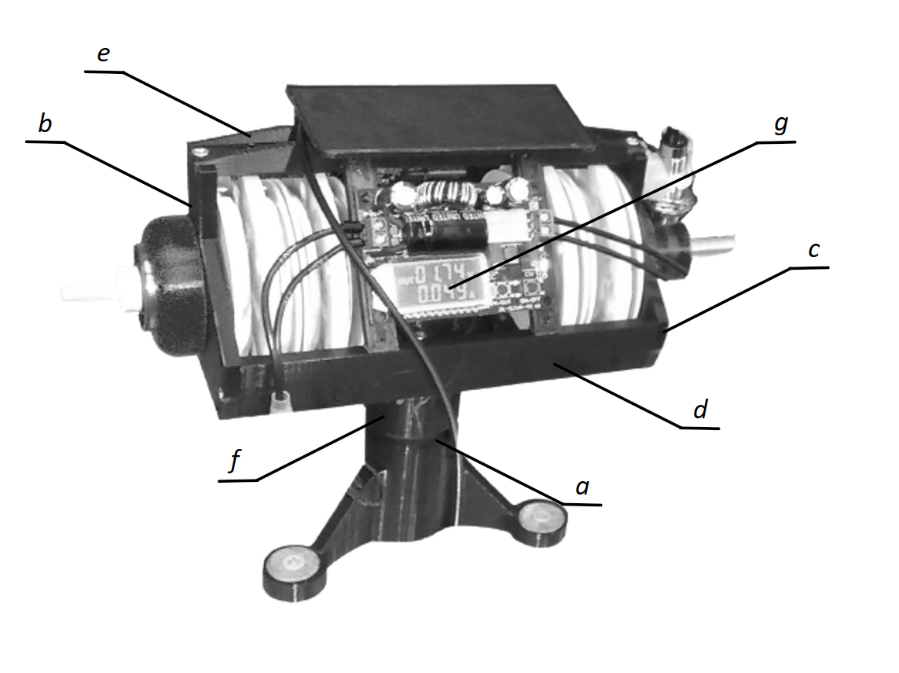
\includegraphics[width=0.4\textwidth]{../_images/housing.png}
  \caption{Housing assembly}
  \label{img:housing}
\end{figure}

The drivetrain assembly is shown in Figure \ref{img:drivetrain}.
It is composed of the central axle (a) that connects four pairs
of inline rotors (b and c) and two pairs of stators (d and e).
The stators are supported by the housing assembly and are
independent of the rotation of the rotor assembly. Connected to
each pair of stators are housing assemblies that contain two
pairs of internally connected full bridge rectifiers potted in
epoxy. Once the generator selection was settled on, mechanical
design and power electronics work began.
\begin{figure}[th]
  \centering
  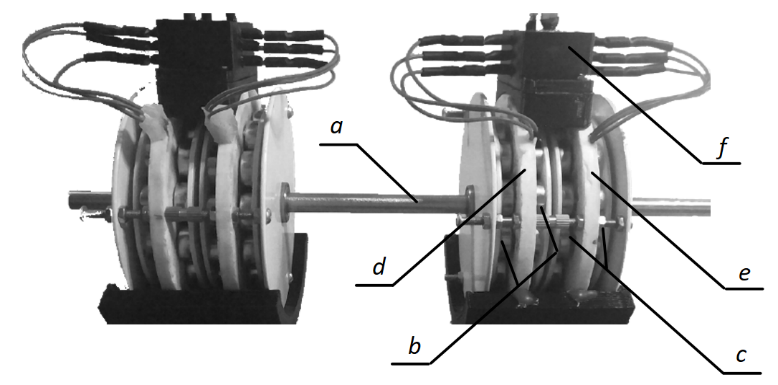
\includegraphics[width=0.4\textwidth]{../_images/drivetrain.png}
  \caption{Drivetrain assembly}
  \label{img:drivetrain}
\end{figure}

Figure \ref{img:schematic} shows the systems power distribution
of the most recent design review.

The load chosen is constructed of a \qty{200}{\W} variable
resistor with coils and contacts throughout to select the
desired resistance for the appropriate wind speed and
scenario. Supplemental resistance was needed for the lower wind
speed and lower load conditions, so additional resistors are
combined in series to acquire these values. The resistance
values used in the load box vary from \qty{45}{\ohm} up to
\qty{420}{\ohm}. A relay bank controlled by a separate Arduino
from the turbine is used to select the load by closing the
contacts on the desired resistor value. The Arduino is
receiving commands from the turbine through an optically
isolated TX and RX line. This Arduino will send commands to
the turbine if a manual shutdown is required.
\begin{figure}[bh]
  \centering
  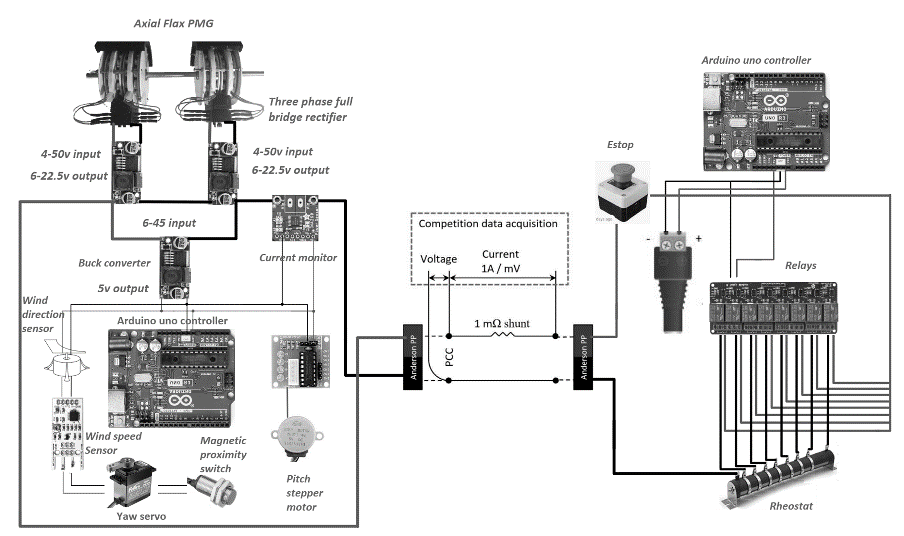
\includegraphics[width=\textwidth]{../_images/schematic.png}
  \caption{Pictorial schematic of the turbine's control and load
    power distribution}
  \label{img:schematic}
\end{figure}

\subsection{Control Theory}
The pitch control scheme is made up of a methodology called
Fuzzy Logic, as shown in Figure \ref{img:control}. The
tachometer measures the RPM of the turbine
and then the controller determines how far away that the
current RPM is from the desired RPM of the turbine. The
previous RPM record is also taken into consideration when
determining whether to make a pitch adjustment or not. If the
turbine is rotating too slowly, but is speeding up, the
algorithm will wait another cycle to see if the pitch has
continued to increase the RPM, and if not, it will then make
an appropriate adjustment based on how far away from the
desired RPM it is. If the turbine RPM is within acceptable
bounds to the desired RPM, then no adjustments will be made.

The tachometer utilizes a Hall effect sensor that counts the
number of pulses it receives, which happens once per
revolution, and calculated the period it takes for 20
revolutions to occur and determines the RPM from this math.
There is a timeout scenario where if 20 revolutions have not
been completed in 5 seconds the loop will break and the RPM
will still be calculated, just with less accuracy because the
time period over fewer revolutions will be averaged.

\onecolumn
\begin{figure}[th]
  \centering
  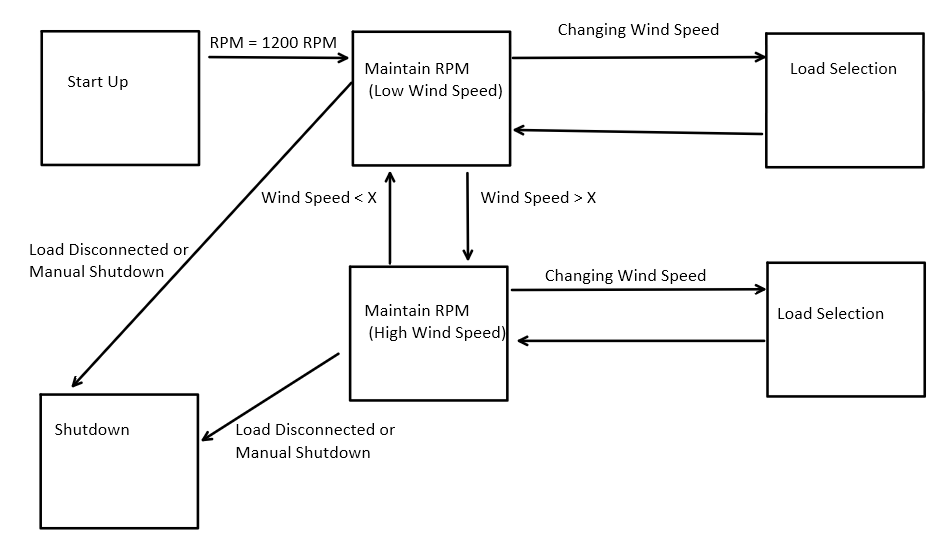
\includegraphics[width=\textwidth]{../_images/control.png}
  \caption{Canonical control model}
  \label{img:control}
\end{figure}
\twocolumn

A current sensor must be used to determine if the load has
been disconnected from the turbine. An ADA260 module
communicates with the Arduino via an I2C connection. When the
load goes above \qty{50}{\mA} the load is detected, and any
drop below that will trigger the pitch to adjust to slow the
blades down to a stop. The minimum load expected at a wind
speed of \qty{5}{\m\per\s} is around \qty{80}{\mA} so this is
not something that could be accidentally tripped.

The wind speed sensor determines the wind speed utilizing the
``hot wire'' method. This method heats up a wire and as the
wind passes by, it cools the wire off changing its resistance
and the voltage across it. The voltage is read by the Arduino
and then the Arduino can determine the wind speed the sensor is
experiencing.

Delays are important for the pitch control system because it
takes some time for the system to stabilize and the RPM to
cease any fluctuations. The problem with using the built-in
delay functions is that the Arduino cannot do anything else
while this is happening. A modified delay function was made so
that crucial measurements can be made in this idle time to
allow action to be taken if something doesn't look right. The
current is monitored so if the load is disconnected, the
turbine can immediately begin slowing down to prevent over
speeding the turbine and damaging both the physical and
electrical components.

Currently, the pitch control mechanism is adjusted by a stepper
motor, but through testing it has been noticed that the stepper
motor has a few flaws, being it is slow, and it draws a lot of
current. The stepper motor takes more than 20 seconds to move
from one extreme pitch setting to the other. This affects the
RPM when the load is disconnected because the elimination of
torque due to the load results in the turbine increasing by
several hundred RPM during disconnects. With faster pitching
speeds, this RPM overshoot can be minimized. Because the
stepper motor draws around \qty{300}{\mA} the added load during
pitch adjustments slows the blades down and results in more
time needed for the RPM to stabilize after pitch adjustments
are made. It is being considered to change to a DC motor with a
gearbox and H-bridge configuration which alleviates both
concerns in preliminary testing, with the current selection
having more speed while also drawing less current.

\subsection{Voltage Regulation Description}
The voltage regulation system consists of four axial flux
motors tied in series after their respective voltages have
been rectified. This allows for a high KV rating which is
important for low RPM operation of the Arduino. Two adjustable
buck converters are each attached to two rectifier outputs in
series, limited to \qty{22.5}{\V}. When these two buck
converters are connected in series the system total voltage is
limited to \qty{45}{\V}. Two buck converters connected in
series are needed because each is rated for \qty{52}{\V},
allowing for a maximum turbine voltage of \qty{104}{\V} which
is achieved at around \qty{2400}{RPM} or twice the
\qty{1200}{RPM} normal operational speed of the turbine. The
initial intent was to achieve a high voltage quickly to run the
Arduino at low RPMs and sustain it for the manual and
emergency stop scenarios so that the turbine could
automatically restart.

Unfortunately, through testing it was discovered that each of
the buck convertors requires a minimum of \qty{4.5}{\V} to
operate, which now brings the minimum operating voltage to
\qty{9}{\V} instead of the \qty{5}{\V} that the Arduino needs
to say alive. Applying the KV rating formula from
\eqref{eq:KV} gives \qty{216}{RPM} as the minimum rotational
speed for turbine's control system to operate. This would
require the normal operational speed of the turbine to go up by
\qtyrange{960}{2160}{RPM}, this is according to CWC 10\% of
maximum speed requirement during load-disconnect shutdown
procedure.

Because during the emergency shutdown it takes time for the
system to respond to the load being disconnected, there exists
a time were RPM continuous to rise. Having only \qty{240}{RPM}
buffer before buck converters' operational limit is surpassed
by overvoltage, brings a self-restart operation of the turbine
to the unpredictable operation conditions, where buck converter
failure is very likely.

From observation, the system can surpass the \qty{240}{RPM}
buffer zone faster than the control system can respond to slow
itself down. At this time, the team was not able to find a
solution for this problem and turbine is designed to be
manually restarted after emergency stop. A faster pitch
control system is being designed, using DC motor, gear box and
limit switches to prevent over travel. More tests are needed
to determine if new pitch control scenario will deliver the
self-restart capability.


\subsection{Software Development}
A lot of adjustments and improvements have been made to the
pitch control algorithm. At first there were five choices the
program could make to adjust the pitch: no adjustment and
small/big adjustment to make the blades go faster/slower.
Later it was observed that if the blades were accelerating
towards the desired RPM, there may not need to be any
adjustment made. The pitch adjustment motor used also requires
power to use, and so with every pitch adjustment, not only is
there a delay required due to the change in aerodynamics, but
the additional load that the motor requires will slow the
turbine down as well, which may need additional time to allow
for RPM stabilization. As the wind speed increases, because
there is more power in the wind, the turbine reacts more
quickly to pitch changes, and so the delay times must be
shortened as wind speed increases. The turbine is also more
sensitive to pitch changes at high wind speeds and RPM, and so
the adjustments made are smaller as the wind speed increase.
If the turbine is trying to supply more power than it can
extract from the wind, which would cause the RPM to drop due to
blade stall. The blades will pitch back to a previous setting
to try and reduce or save the stall condition if too many
``large pitch adjustment faster'' conditions occur
consecutively. While the delay functions built into the
Arduino software work well, the current cannot be measured
during this delay time, and so if the load is disconnected it
could be up to three seconds before it is noticed by the
software, which could cause the blades to overspeed. A
modified delay function had to be created so that sufficient
delays could still be implemented, and the current could be
checked in case of a disconnect, immediately pitching the
blades back and breaking the turbine.

Wind speed measurement has been more difficult than it was
anticipated. The Rev C wind speed sensor is very sensitive at
low wind speeds, but at high wind speeds the voltage it sends
out only varies by a couple hundredths of a volt per meter per
second of wind. This made it challenging to know exactly what
the wind speed was so a lot of measurements are taken and
averaged and then compared with previous wind speed
measurements to try and verify if the wind speed is constant
or it is changing to a higher or lower speed.

\end{document}
